\chapter{识别物质}\label{ch:g7:identifying-substances}

在一起小型谜案的现场，发现了一张用黑色水性笔写的皱巴巴的便条，
同时在三个不同的袋子里找到了三支水性笔。
肉眼看去，三种墨水都是黑色的。
法庭化学家只需一条纸带、少量水和半小时，
就能判断便条是哪支笔写的。化学家识别物质，
不是看它们的外观，而是看它们在为之选定的试验中表现出什么性质。

\begin{recall}
\omterm{def:g6:pure-substances-and-mixtures:species}{化学物种}是某一种特定的物质；\omterm{def:g6:pure-substances-and-mixtures:pure-substance}{纯净物}只含一种
\omterm{def:g6:pure-substances-and-mixtures:mixture}{混合物}则含有多种
（见\cref{ch:g6:pure-substances-and-mixtures}）。有些物质易溶于\omterm{def:g6:solutions-and-solubility:solute}{溶剂}，
有些则难溶甚至不溶，每种物质都有各自的
\omterm{def:g6:solutions-and-solubility:solubility}{溶解度}（见\cref{ch:g6:solutions-and-solubility}）。
\end{recall}

\section{什么是特征检验}

\begin{definition}[特征检验与试剂]\label{def:g7:identifying-substances:characteristic-test}
对某一\omterm{def:g6:pure-substances-and-mixtures:species}{化学物种}的\emph{特征检验}\index{特征检验}是一种简单的实验，
它对该物种给出可见的结果，
而对同一情境中遇到的其他物种则不会。它使用专为此选定的物质，
称为
\emph{试剂}\index{试剂}。
\end{definition}


\begin{method}[进行特征检验]\label{met:g7:identifying-substances:run}
\begin{enumerate}
  \item 取少量待检验的物质作为样品。
  \item 加入\omterm{def:g7:identifying-substances:characteristic-test}{试剂}，或使其与样品接触，
        按试验所述的方式操作。
  \item 观察：颜色变化、变浑浊、出现火焰或声音。
  \item 得出结论：若出现预期的结果，则试验为\emph{阳性}，
        否则为\emph{阴性}。
  \item 对已知不含该物种的样品（即空白样）做同样的试验，
        其结果必须仍为阴性，否则
        试验结果便无法说明任何问题。
\end{enumerate}
\end{method}

\section{四种经典检验}

\begin{proposition}[二氧化碳使石灰水变浑浊]\label{prop:g7:identifying-substances:limewater}
石灰水是一种澄清、无色的溶液。当二氧化碳
通入其中时，石灰水变为乳白色浑浊。通过吸管呼出的\omterm{def:g4:air-a-mixture-of-gases:air}{空气}
能使石灰水变浑浊；抽入其中的新鲜\omterm{def:g4:air-a-mixture-of-gases:air}{空气}
则几乎不能使其变浑浊。
\end{proposition}

\begin{omfigure}
\begin{tikzpicture}[font=\small, scale=1.25]
  % generating tube, stoppered
  \pic[transform shape] at (0,0) {testtube={0.35}{omWater!80}};
  \fill[black!65] (-0.27,2.8) rectangle (0.27,3.15);
  \foreach \y in {0.4,0.65,0.85} \draw[black!55] (0.05,\y) circle (0.04);
  \pic[transform shape] at (0,2.9) {deliverytube={1.9}{-2.3}};
  % limewater tube
  \pic[transform shape] at (1.9,0) {testtube={0.6}{white!85!black}};
  \foreach \x/\y in {1.88/0.75,1.95/1.0,1.85/1.25,1.92/1.5} \draw[black!55] (\x,\y) circle (0.04);
  \draw[<-, omProp, thick] (-0.3,0.5) -- (-1.2,0.8) node[left, text=black, align=right]
    {产生气体的 \\反应};
  \draw[<-, omProp, thick] (2.2,1.2) -- (3.0,1.4) node[right, text=black, align=left]
    {石灰水变浑浊：\\该气体是 \\二氧化碳};
\end{tikzpicture}

{\small 石灰水检验。第一支试管中产生的气体通入
石灰水中；若石灰水变浑浊，则该气体为
二氧化碳。}
\end{omfigure}

\begin{proposition}[水使无水硫酸铜变蓝]\label{prop:g7:identifying-substances:copper-sulfate}
无水硫酸铜是一种白色粉末。一滴水即可使其
立即变蓝。该试验表明，待测样品中有水存在，无论是液体
还是潮湿的固体——并不说明该液体就是纯水。
\end{proposition}

\begin{omfigure}
\begin{minipage}[b]{0.48\linewidth}\centering
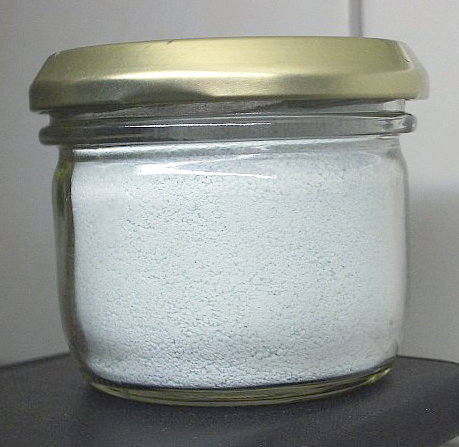
\includegraphics[width=\linewidth,height=4.2cm,keepaspectratio]{images/book1/cuso4-anhydrous.jpg}

{\small 无水硫酸铜：白色粉末。照片：W.~Oelen，
CC BY-SA 3.0。}
\end{minipage}\hfill
\begin{minipage}[b]{0.48\linewidth}\centering
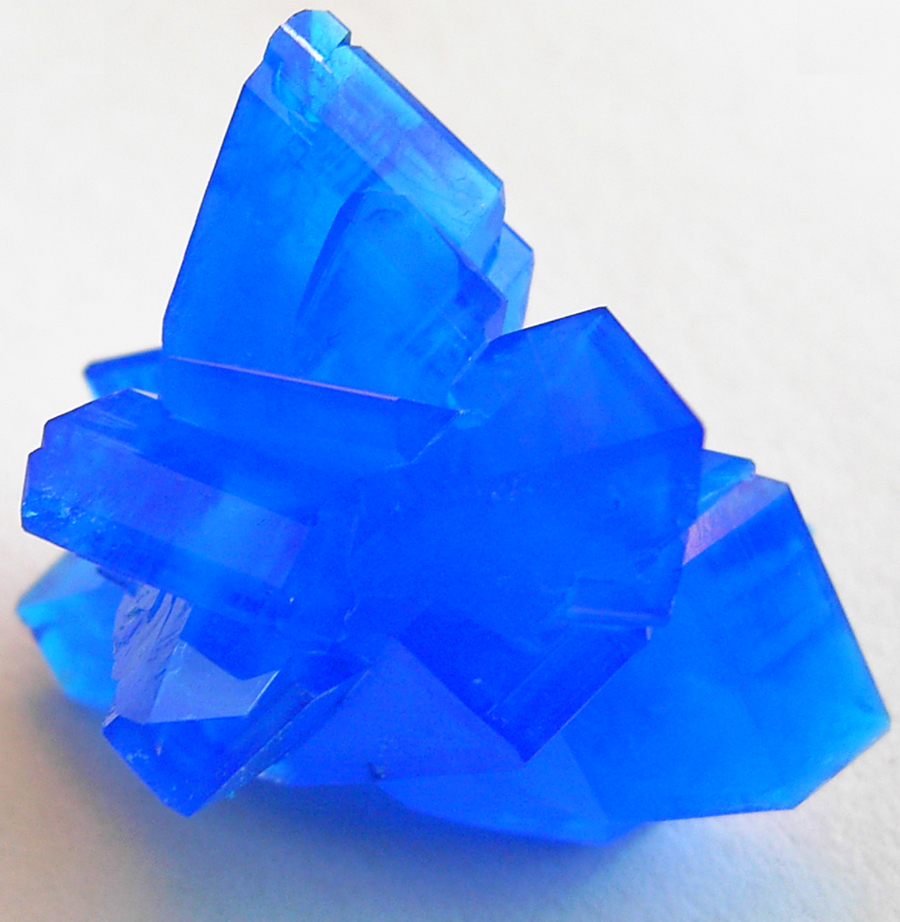
\includegraphics[width=\linewidth,height=4.2cm,keepaspectratio]{images/book1/cuso4-hydrated.jpg}

{\small 遇水变蓝；这些晶体含有水。照片：Stephanb，
CC BY-SA 3.0。}
\end{minipage}
\end{omfigure}

\begin{safety}{\ghs[0.82cm]{GHS05}\ghs[0.82cm]{GHS07}\ghs[0.82cm]{GHS09}}
% ledger: ghs:CuSO4
硫酸铜：误食有害，刺激皮肤（GHS07）；
可严重损伤眼睛（GHS05）；对水生生物毒性很大，
并具有长期影响（GHS09）。佩戴护目镜和手套；废弃物
须收集，切勿倒入水槽。
\end{safety}

\begin{proposition}[氧气使带火星的木条复燃]\label{prop:g7:identifying-substances:splint}
将木条点燃后吹灭，使其只剩红热的余烬。
将带火星的木条伸入盛有氧气的试管中，木条
重新燃起火焰。
\end{proposition}

\begin{proposition}[氢气燃烧发出尖锐的爆鸣声]\label{prop:g7:identifying-substances:pop}
将点燃的木条靠近盛有氢气的小试管口，
发出一声短促、尖锐的“噗”声：氢气
立即与\omterm{def:g4:air-a-mixture-of-gases:air}{空气}中的氧气\omterm{def:g4:what-a-fire-needs:burning}{燃烧}。
\end{proposition}

\begin{omfigure}
\begin{tikzpicture}[font=\small, scale=1.25]
  % splint test for oxygen
  \pic[transform shape] at (0,0) {testtube={0}{white}};
  \draw[brown!60!black, line width=2pt] (0.15,1.6) -- (1.4,3.6);
  \fill[orange!85] (0.15,1.6) circle (0.07);
  \fill[orange!80] (0.12,1.62) .. controls (0.0,1.9) and (0.08,2.1) .. (0.1,2.3)
    .. controls (0.2,2.05) and (0.3,1.85) .. (0.2,1.62);
  \node[anchor=north, align=center] at (0,-0.15) {氧气：\\ 带火星的木条 \\ 复燃};
  % pop test for hydrogen
  \begin{scope}[xshift=4cm]
    \pic[transform shape, rotate=180] at (0,3.1) {testtube={0}{white}};
    \draw[brown!60!black, line width=2pt] (0.05,-0.05) -- (1.3,-0.9);
    \fill[orange!85] (0.05,-0.02) .. controls (-0.05,0.08) and (0.0,0.15) .. (0.02,0.22)
      .. controls (0.08,0.15) and (0.15,0.08) .. (0.1,-0.02);
    \node[font=\small\itshape] at (-0.9,0.15) {噗！};
    \node[anchor=north, align=center] at (0,-1.0) {氢气：\\ 尖锐的爆鸣声 \\ 在管口};
  \end{scope}
\end{tikzpicture}

{\small 左：带火星的木条在氧气中复燃。右：点燃的木条
靠近倒置盛有氢气的试管口，发出尖锐的“噗”声
（氢气比\omterm{def:g4:air-a-mixture-of-gases:air}{空气}轻，所以试管管口朝下放置。）}
\end{omfigure}

\begin{safety}{\ghs[0.82cm]{GHS02}\ghs[0.82cm]{GHS04}}
% ledger: ghs:H2
氢气：极易燃的气体（GHS02），以压缩状态储存在
钢瓶中（GHS04）。做“噗”声试验时只用几毫升，
由教师进行。
\end{safety}

\section{纸色谱法}

\begin{definition}[纸色谱法与色谱图]\label{def:g7:identifying-substances:chromatography}
\emph{纸色谱法}\index{纸色谱法}用于分离
\omterm{def:g6:pure-substances-and-mixtures:mixture}{混合物}中的染料。取少量\omterm{def:g6:pure-substances-and-mixtures:mixture}{混合物}的斑点，点在距纸条底部
附近画好的线上；将纸条底端浸入
\omterm{def:g6:solutions-and-solubility:solute}{溶剂}中，\omterm{def:g6:solutions-and-solubility:solute}{溶剂}缓慢沿纸条上升，携带各种染料一同移动，
其中有的染料移动较快。当\omterm{def:g6:solutions-and-solubility:solute}{溶剂}上升至接近顶端时，
取出纸条并晾干，所得即为
\emph{色谱图}\index{色谱图}。
\end{definition}

\begin{omfigure}
\begin{tikzpicture}[font=\small, scale=1.3]
  % the strip in a beaker of solvent
  \pic[transform shape] at (0,0) {beaker={0.12}{omWater!80}};
  \fill[white] (-0.42,0.06) rectangle (0.42,2.2);
  \fill[omWater!80] (-0.42,0.06) rectangle (0.42,0.24);
  \draw[omGlass, line width=0.6pt] (-0.42,0.06) rectangle (0.42,2.2);
  \draw[black!60, line width=0.4pt] (-0.42,0.42) -- (0.42,0.42);
  \fill[black!80] (0,0.42) circle (0.07);
  \shade[ball color=black!20] (0,2.27) circle (0.08);
  \draw[black!50, line width=1.2pt] (-1.1,2.27) -- (1.1,2.27);
  \node[anchor=north, align=center] at (0,-0.15) {开始时};
  \draw[<-, omProp, thick] (0.1,0.5) -- (1.3,0.8) node[right, text=black]
    {铅笔线上的墨迹};
  \draw[<-, omProp, thick] (1.0,2.27) -- (1.3,2.5) node[right, text=black]
    {固定纸条的玻璃棒};
  \draw[<-, omProp, thick] (0.75,0.15) -- (1.3,0.25) node[right, text=black]
    {溶剂，在线的下方};
  % the chromatogram
  \begin{scope}[xshift=6.2cm]
    \pic[transform shape] at (0,0) {tlcplate};
    \draw[black!50, dashed] (-0.7,2.7) -- (0.7,2.7);
    \fill[blue!70] (0,1.0) ellipse (0.13 and 0.09);
    \fill[red!70] (0,1.7) ellipse (0.13 and 0.09);
    \fill[yellow!80!orange] (0,2.35) ellipse (0.13 and 0.09);
    \node[anchor=north, align=center] at (0,-0.15) {色谱图};
    \draw[<-, omProp, thick] (0.75,2.7) -- (1.3,2.85) node[right, text=black]
      {溶剂上升的高度};
    \draw[<-, omProp, thick] (0.2,1.7) -- (1.3,1.7) node[right, text=black]
      {三种染料：墨水是混合物};
  \end{scope}
\end{tikzpicture}

{\small 黑色墨水的纸色谱。\omterm{def:g6:solutions-and-solubility:solute}{溶剂}沿纸条上升，
使墨水分离为三种染料。}
\end{omfigure}

\begin{method}[读取色谱图]\label{met:g7:identifying-substances:read}
\begin{enumerate}
  \item 数一数各起点上方的斑点：一个斑点说明为一种染料；
        两个或更多斑点则为染料的\omterm{def:g6:pure-substances-and-mixtures:mixture}{混合物}。
  \item 比较高度：同一\omterm{def:g7:identifying-substances:chromatography}{色谱图}中，同一种染料总是
        上升到相同的高度。与已知染料处于同一高度的斑点，
        很可能就是该种染料。
  \item 应使用铅笔画线，切勿用墨水：墨水本身也会
        被\omterm{def:g6:solutions-and-solubility:solute}{溶剂}分离。
\end{enumerate}
\end{method}

\begin{example}[糖果中的染料]\label{ex:g7:identifying-substances:sweets}
取糖果的彩色糖衣，刮入少量水中，
点在纸条上，旁边同时点上糖果中允许使用的食品染料。
\omterm{def:g7:identifying-substances:chromatography}{色谱图}表明，绿色糖衣含有一种黄色染料和一种
蓝色染料，两者都在允许使用的染料之中。
\end{example}


\section{阅读特征检验表}

\begin{proposition}[特征检验表]\label{prop:g7:identifying-substances:bank}
化学家把常用的检验方法整理成一张表，称为“检验表”，
该表由左至右阅读：
\begin{center}
\small
\begin{tabular}{llll}
\hline
所检测的\omterm{def:g6:pure-substances-and-mixtures:species}{化学物种} & \omterm{def:g7:identifying-substances:characteristic-test}{试剂}或检验 & 阳性结果 & \\
\hline
二氧化碳 & 石灰水 & 石灰水变浑浊 & \\
水 & 无水硫酸铜 & 白色变为蓝色 & \\
氧气 & 带火星的木条 & 木条复燃 & \\
氢气 & 点燃的木条 & 尖锐的“噗”声 & \\
\omterm{def:g6:pure-substances-and-mixtures:mixture}{混合物}中的染料 & \omterm{def:g7:identifying-substances:chromatography}{纸色谱法} & 每种染料一个斑点 & \\
\hline
\end{tabular}
\end{center}
\end{proposition}

\begin{remark}[检验不能说明什么]\label{rem:g7:identifying-substances:limits}
阳性检验只能证明该\omterm{def:g6:pure-substances-and-mixtures:species}{化学物种}存在，而不能证明它
是单独存在的：能使硫酸铜变蓝的液体含有水，但它
也可能是咸水或橙汁。阴性检验只能说明该\omterm{def:g6:pure-substances-and-mixtures:species}{化学物种}
不存在，或其含量太少而无法显示。
\end{remark}

\begin{omfigure}
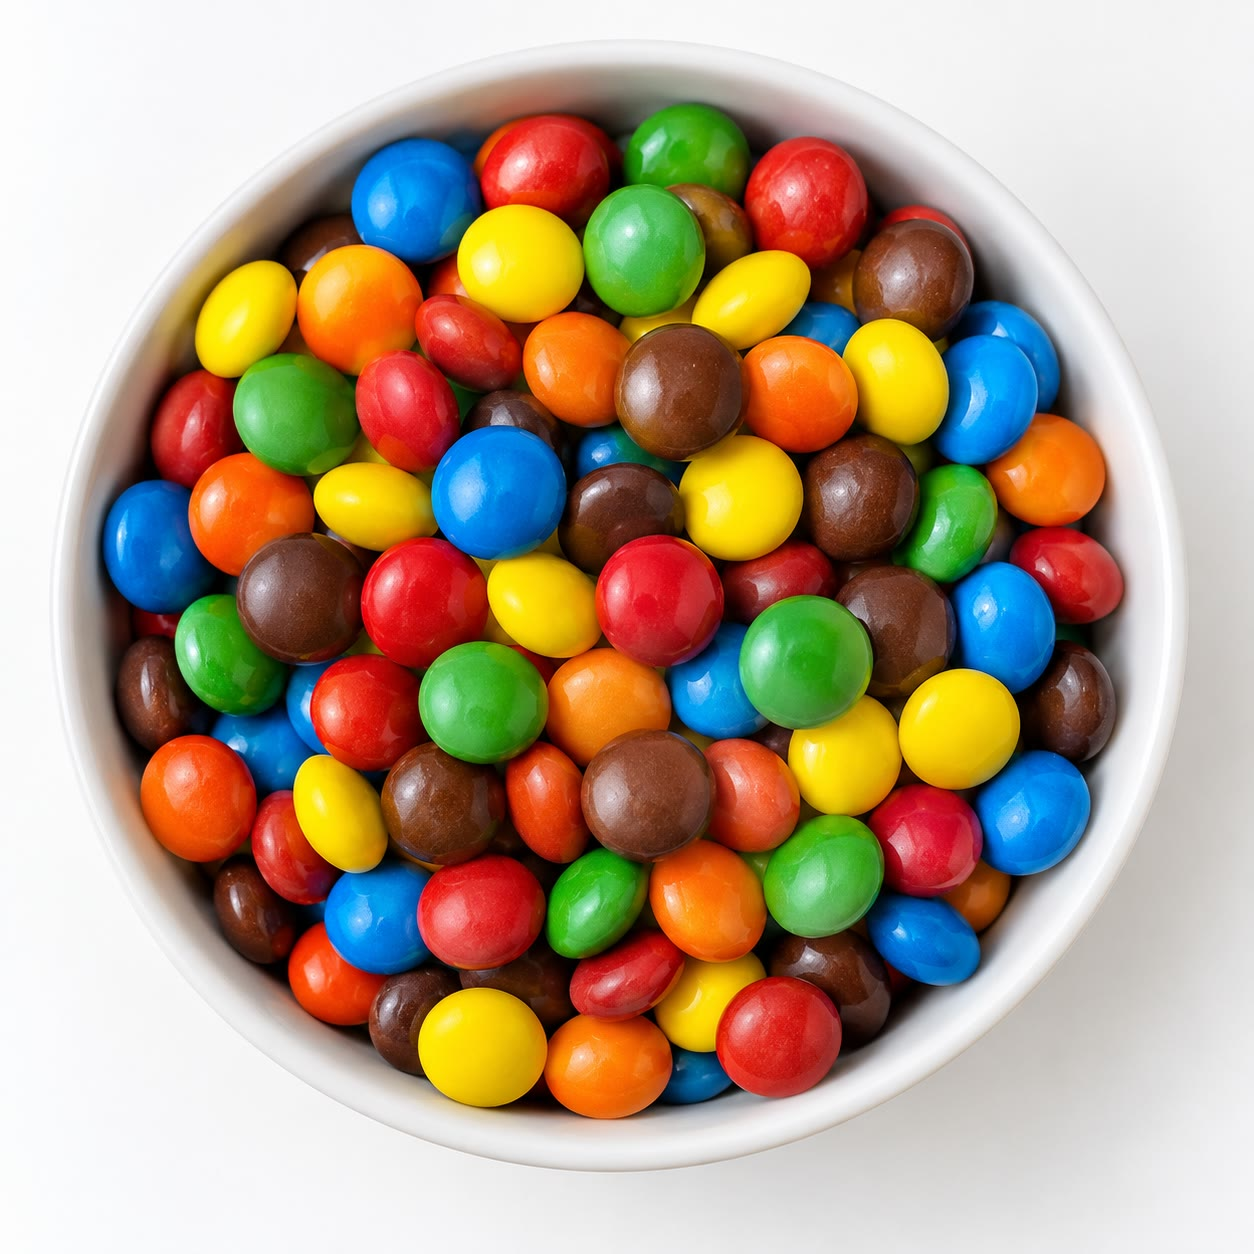
\includegraphics[width=0.32\linewidth]{images/book1/ai/g7-sweets.jpg}

{\small 糖衣糖果：其颜色是染料的\omterm{def:g6:pure-substances-and-mixtures:mixture}{混合物}，
可用色谱法将其分离。}
\end{omfigure}

\begin{omfigure}
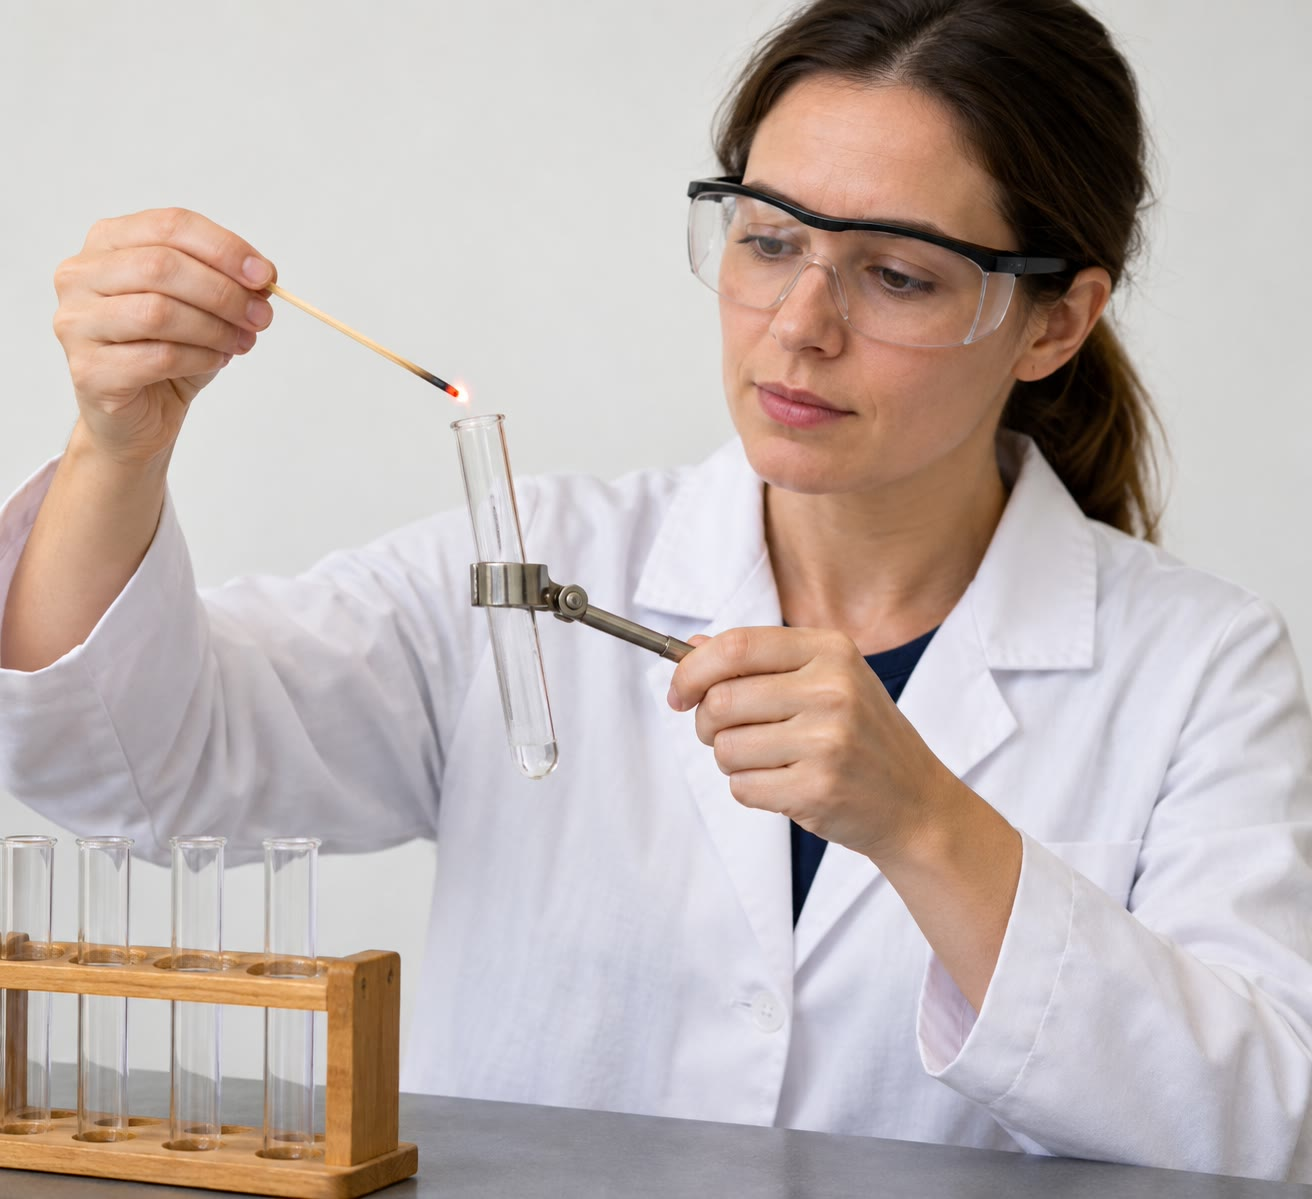
\includegraphics[width=0.36\linewidth]{images/book1/ai/g7-splint-teacher.jpg}

{\small 教师用带火星的木条检验一种气体。}
\end{omfigure}

\section{练习}

\begin{exercise}[$\star$]\label{exo:g7:identifying-substances:1}
用哪种检验可以鉴别二氧化碳？描述其阳性结果。
\end{exercise}

\begin{exercise}[$\star$]\label{exo:g7:identifying-substances:2}
向一种白色粉末上滴加某种液体，粉末变为蓝色。
这说明该液体中含有什么？
\end{exercise}

\begin{exercise}[$\star$]\label{exo:g7:identifying-substances:3}
将带火星的木条伸入一瓶气体中，木条复燃。该瓶中
装的是什么气体？
\end{exercise}

\begin{exercise}[$\star$]\label{exo:g7:identifying-substances:4}
\omterm{def:g7:identifying-substances:chromatography}{纸色谱法}中，起始线为什么用铅笔画，
而不用墨水画？
\end{exercise}

\begin{exercise}[$\star\star$]\label{exo:g7:identifying-substances:5}
起始线为什么必须高于烧杯中
\omterm{def:g6:solutions-and-solubility:solute}{溶剂}的液面？
\end{exercise}

\begin{exercise}[$\star\star$]\label{exo:g7:identifying-substances:6}
某绿色墨水的\omterm{def:g7:identifying-substances:chromatography}{色谱图}上有两个斑点，一个与黄色标准染料
处于同一高度，另一个与蓝色标准染料处于同一高度。该
绿色墨水是\omterm{def:g6:pure-substances-and-mixtures:pure-substance}{纯净物}吗？它是由什么组成的？
\end{exercise}

\begin{exercise}[$\star\star$]\label{exo:g7:identifying-substances:7}
利用检验题库，若要证明某反应放出的气体是氢气，
应选用哪种检验？你预期会看到什么现象？
\end{exercise}

\begin{exercise}[$\star\star$]\label{exo:g7:identifying-substances:8}
呼出的气体使石灰水变浑浊的速度远快于新鲜\omterm{def:g4:air-a-mixture-of-gases:air}{空气}。
这说明呼出的气体有何特点？
\end{exercise}

\begin{exercise}[$\star\star$]\label{exo:g7:identifying-substances:9}
一种澄清的液体使无水硫酸铜变蓝。萨姆得出结论：
“这是纯净的水。”请解释萨姆为什么错了。
\end{exercise}

\begin{exercise}[$\star\star$]\label{exo:g7:identifying-substances:10}
观察本章的黑色墨水\omterm{def:g7:identifying-substances:chromatography}{色谱图}，
该墨水含有几种染料？哪一种上升得最高？
\end{exercise}

\begin{exercise}[$\star\star\star$]\label{exo:g7:identifying-substances:11}
三瓶气体分别是氧气、氢气和二氧化碳，但标签
已脱落。请在纸上设计检验方案，以确定每瓶气体，
并使所用的检验次数尽可能少。
\end{exercise}

\begin{exercise}[$\star\star\star$]\label{exo:g7:identifying-substances:12}
某同学用石灰水检验一种气体，未观察到明显现象。
请给出两种可能的解释，并说明有助于判断的对照实验。
\end{exercise}

\section{问题：伪造的字条}

\begin{problem}[{周末问题——一张黑色水笔书写的字条、三支可疑的笔，
三个无标签的气瓶以及一套检验题库}]
\label{pb:g7:identifying-substances:1}
某学校实验室受托协助解决两个小谜题。第一个是：
一张用黑色水笔书写的字条，需与三支黑色笔中的一支相对应，
三支笔分别编号为 1、2 和 3。从字条和每支笔上各取一滴墨水，
点在同一条纸带上，再用水将纸带展开。
\omterm{def:g7:identifying-substances:chromatography}{色谱图}如下所示。
\begin{center}
\begin{tikzpicture}[font=\small, x=1cm, y=1cm]
  \fill[white] (0,0) rectangle (6,4);
  \draw[omGlass, line width=0.6pt] (0,0) rectangle (6,4);
  \draw[black!60] (0,0.5) -- (6,0.5);
  \draw[black!50, dashed] (0,3.6) -- (6,3.6);
  \foreach \x/\lab in {0.9/字条, 2.3/笔 1, 3.7/笔 2, 5.1/笔 3}
    \node[anchor=north] at (\x,-0.05) {\lab};
  % note: three dyes
  \fill[blue!70] (0.9,1.2) ellipse (0.18 and 0.1);
  \fill[red!70] (0.9,2.2) ellipse (0.18 and 0.1);
  \fill[yellow!80!orange] (0.9,3.1) ellipse (0.18 and 0.1);
  % pen 1: two dyes
  \fill[blue!70] (2.3,1.2) ellipse (0.18 and 0.1);
  \fill[black!70] (2.3,2.7) ellipse (0.18 and 0.1);
  % pen 2: same three as the note
  \fill[blue!70] (3.7,1.2) ellipse (0.18 and 0.1);
  \fill[red!70] (3.7,2.2) ellipse (0.18 and 0.1);
  \fill[yellow!80!orange] (3.7,3.1) ellipse (0.18 and 0.1);
  % pen 3: three dyes, other heights
  \fill[violet!70] (5.1,0.9) ellipse (0.18 and 0.1);
  \fill[red!70] (5.1,1.8) ellipse (0.18 and 0.1);
  \fill[green!60!black] (5.1,2.6) ellipse (0.18 and 0.1);
  \node[anchor=west, font=\footnotesize] at (6.1,3.6) {溶剂前沿};
  \node[anchor=west, font=\footnotesize] at (6.1,0.5) {起始线};
\end{tikzpicture}
\end{center}

\medskip
\noindent\textbf{第一部分——\omterm{def:g7:identifying-substances:chromatography}{色谱图}。}
\begin{enumerate}
  \item 为什么四种墨水要点在同一条纸条上，
        并一起展开？
  \item 该便条上的墨水是\omterm{def:g6:pure-substances-and-mixtures:pure-substance}{纯净物}还是\omterm{def:g6:pure-substances-and-mixtures:mixture}{混合物}？请说明理由。
  \item 1 号笔的墨水含有几种染料？
        1 号笔是否可能写过该便条？
  \item 3 号笔的墨水也含有三种染料，
        为什么它不可能写出该便条？
  \item 哪支笔与该便条的墨迹相符？
        请利用斑点的高度加以说明。
\end{enumerate}

\medskip
\noindent\textbf{第二部分——三个气瓶。}
第二个谜题：三个小气瓶 X、Y 和 Z 的标签已脱落，
它们分别装有氧气、氢气和二氧化碳。用试管从每个气瓶中各收集少量气体。
气体 X 能使带火星的木条复燃。气体 Y 遇点燃的木条发出爆鸣声。
气体 Z 能使澄清石灰水变浑浊。
\begin{enumerate}[resume]
  \item 写出气体 X 的名称。
  \item 写出气体 Y 的名称。
  \item 写出气体 Z 的名称。
  \item 检验气体 Z 之前，同学用相同时间将普通\omterm{def:g4:air-a-mixture-of-gases:air}{空气}通入同一石灰水中，
        石灰水仍然澄清。这一步骤叫什么？
        它为结论提供了什么补充？
\end{enumerate}

\medskip
\noindent\textbf{第三部分——检验题库。}
\begin{enumerate}[resume]
  \item 在便条旁发现一种无色液体，它使无水硫酸铜变蓝。
        请写出所用的检验方法，
        并说明结果表明了什么。
  \item 该结果能否证明这种液体是纯水？请说明理由。
  \item 请对第一个谜题作出结论：该便条的墨水含有几种染料，
        是哪支笔所写？
\end{enumerate}
\end{problem}
